\documentclass[border=4pt]{standalone}
% Preámbulo común de las figuras. Cada figura es un documento standalone
% que se compila a SVG con scripts/build_figures.sh
\usepackage[utf8]{inputenc}
\usepackage{amsmath}
\usepackage{tikz}
\usepackage[american, siunitx]{circuitikz}
\usetikzlibrary{arrows.meta,calc,decorations.pathmorphing,patterns}
\tikzset{
  >={Stealth[length=2.2mm]},
  eje/.style={->, thin},
  hilo/.style={thick},
}

\begin{document}
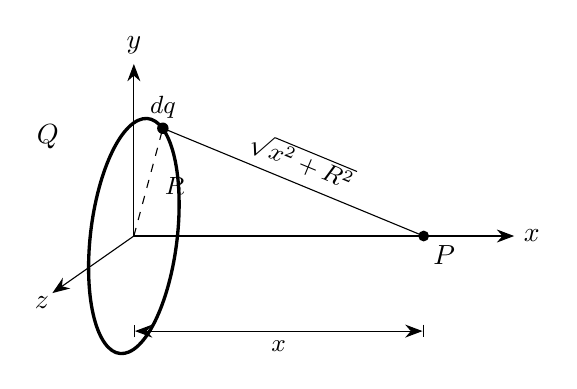
\begin{tikzpicture}[scale=1.15]
  \draw[eje] (0,0) -- (4.2,0) node[right]{$x$};
  \draw[eje] (0,0) -- (0,1.9) node[above]{$y$};
  \draw[eje] (0,0) -- (-0.9,-0.63) node[below left, inner sep=1pt]{$z$};
  \begin{scope}[cm={-0.4,-0.28,0,1,(0,0)}]
    \draw[very thick] (0,0) circle (1.25);
  \end{scope}
  \coordinate (dq) at (0.32,1.19);
  \coordinate (P) at (3.2,0);
  \draw[dashed] (0,0) -- (dq);
  \node[font=\small] at (0.45,0.55) {$R$};
  \fill (dq) circle (1.8pt) node[above, font=\small]{$dq$};
  \draw[thin] (dq) -- node[above, sloped, font=\small]{$\sqrt{x^2+R^2}$} (P);
  \fill (P) circle (1.7pt) node[below right]{$P$};
  \draw[|<->|, thin] (0,-1.05) -- node[below, font=\small]{$x$} (3.2,-1.05);
  \node at (-0.95,1.1) {$Q$};
\end{tikzpicture}
\end{document}
